\documentclass[
    journal=jctcce,
    layout=twocolumn
]{achemso}

\setkeys{acs}{
	abbreviations = false,
	articletitle  = false,
	keywords      = false,
	maxauthors    = 10,
	super         = true
}

% Comment below before submitting:
\let\titlefont\undefined
\usepackage[fontsize=11pt]{scrextend}
\usepackage[hidelinks,colorlinks,citecolor=blue]{hyperref}
%\flushbottom
% Up to this point

\usepackage{amsmath}
\usepackage{amssymb}
\usepackage[T1]{fontenc}
%
\usepackage{natbib}
\usepackage{natmove}
%
\usepackage{graphicx}
\DeclareGraphicsExtensions{.pdf,.eps,.png}
\graphicspath{{Figures/}}
\usepackage[outdir=Figures/]{epstopdf}
%
\usepackage[table]{xcolor}
\definecolor{lightgray}{gray}{0.85}
%
\usepackage{tikz}
%
\usepackage{array}
\newcolumntype{L}{>{$}l<{$}}
\newcolumntype{C}{>{$}c<{$}}
\newcolumntype{R}{>{$}r<{$}}
%
\newcommand{\mt}[1]{\boldsymbol{\mathbf{#1}}}   % matrix symbol
\newcommand{\vt}[1]{\boldsymbol{\mathbf{#1}}}   % vector symbol
\newcommand{\tr}[1]{#1^\text{t}}                % transposition
\newcommand{\diff}[2]{\frac{\partial #2}{\partial #1}} % derivative
%\newcommand{\diff}[2]{\nabla_{#1}{#2}} % derivative
%\newcommand{\diff}[2]{\partial_{#1}{#2}} % derivative
\newcommand{\avg}[1]{\overline{#1}}             % average

\newcommand{\dof}{i}   % index for each degree of freedom
\newcommand{\Liu}{i\!L}

%\listfiles

\author{Charlles R. A. Abreu}
\email{abreu@eq.ufrj.br}
\affiliation{Chemical Engineering Department, Escola de Quimica, Universidade Federal do Rio de Janeiro, Rio de Janeiro, RJ 21941-909, Brazil}
\alsoaffiliation{Department of Chemistry, New York University, New York, New York 10003, USA}

\author{Mark E. Tuckerman}
\email{marktuckerman@nyu.edu}
\affiliation{Department of Chemistry, New York University, New York, New York 10003, USA}
\alsoaffiliation{Courant Institute of Mathematical Sciences, New York University, New York, New York 10012, USA}
\alsoaffiliation{NYU-ECNU Center for Computational Chemistry at NYU Shanghai, Shanghai 200062, China}


\title{Alternative Splitting Schemes for Multiple Time-Scale Integrators}

\abbreviations{i.i.d., MC, MD, CLT, OBM, MSE, FEP, BAR, WHAM, MBAR, MICS}

\keywords{Free Energy Computation, Reweighting, Multistate, Uncertainty Estimation}

\begin{document}

%\begin{tocentry}
%Graphical Abstract
%\end{tocentry}

%\tableofcontents

\begin{abstract}
To be included.
\end{abstract}

\section{Introduction}
\label{sec:introduction}

Problems in the evaluation of configurational properties such as the atomic virial have been reported \cite{Andoh_2017}.

\section{Methods}

Consider a system of $N$ particles in $d$ dimensions, whose every configurational degree of freedom $\dof$ has coordinate $q_\dof$, momentum $p_\dof$, and associated mass $m_\dof$.
The system is subject to a potential field $U(q)$ and, therefore, the force acting on $\dof$ is $F_\dof = -\diff{q_\dof}{U}$.
In addition, a set of extended phase-space variables is included so that the original phase space can be dynamically sampled in accordance with some specified statistical ensemble.
If $x$ is a vector comprising all dynamical variables, we can represent the equations of motion which describe a flow through the extended phase space as
\begin{equation}
\label{eq:general equation of motion}
\dot{x} = \Liu x,
\end{equation}
where $\Liu = \xi(x) \cdot \nabla_x$ is a generalized (i.e. non-Hamiltonian) Liouville operator \cite{Tuckerman_1999, Tuckerman_2001, Tuckerman_2006}.

The solution of this equation is formally written as $x_t = e^{t\Liu}x_0$.
However, it is usually necessary to approximate the action of the classical propagator $e^{t\Liu}$ numerically.
This can be done by sequentially applying a split operator $\prod_j e^{\Delta t\Liu_j} \approx e^{\Delta \Liu}$, where $\Delta t = t/n$ and $\sum_j \Liu_j = \Liu$.
This means that $n$ is the number of integration steps and $\Delta t$ is the step size.
According to the Trotter theorem \cite{Trotter_1959}, equality holds when $n \to \infty$ and, therefore, $\Delta t \to 0$.

\subsection{Single Time Scale Integration}

Trying to enable a general discussion about single time-scale (STS) integration methods, we start by partitioning the extended phase-space Liouville operator in Eq.~\eqref{eq:general equation of motion} as
\begin{equation}
\label{eq:STS Liouville Partition}
\Liu = \Liu_\mathrm{move} + \Liu_\mathrm{force} + \Liu_\mathrm{bath},
\end{equation}
where $\Liu_\mathrm{move}$ is the only component which entails changes in the particle coordinates,
$\Liu_\mathrm{force}$ is the only one that depends on the forces, and
$\Liu_\mathrm{bath}$ entails transformations in particle momenta which depend exclusively on the state of extended phase-space variables.
Transformations in such extended variables can occur due to the action of any component in Eq.~\eqref{eq:RESPA Liouville Partition}.

As a simple example, consider a system at constant volume subject to the effect of a ``massive'' set of Nos\'e-Hoover thermostats \cite{Tuckerman_2010}.
In a massive thermostatting method, every degree of freedom is acted upon by an individual thermostat.
In this case, the equations of motion for every degree of freedom $\dof$ are
\begin{subequations}
	\label{eq:NH equations of motion}
	\begin{align}
	& \dot{q}_\dof = v_\dof, \label{eq:NH q} \\
	& \dot{v}_\dof = \frac{F_\dof}{m_\dof} - v_{2,\dof} v_\dof, \quad \mathrm{and} \label{eq:NH v}  \\
	& \dot{v}_{2,\dof} = \tfrac{m_\dof v_\dof^2 - kT}{Q_2}, \label{eq:NH v2}
	\end{align}
\end{subequations}
where $v_\dof = p_\dof/m_\dof$ is the velocity of degree of freedom $\dof$,
$kT$ is the Boltzmann constant multiplied by the temperature of the heat bath,
$v_{2,\dof}$ is an auxiliary variable of the thermostat attached to it, and
$Q_2$ is an inertial parameter whose value is the same for all thermostats.
The Liouville operator which generates the equations above is
\begin{multline}
\label{eq:NH Liouville operator}
\Liu_\mathrm{NH} = \sum_\dof \bigg[ v_\dof \diff{q_\dof}{} + \left(\frac{F_\dof}{m_\dof} - v_{2,\dof} v_\dof \right) \diff{v_\dof}{} + \\
+ \frac{m_\dof v_\dof^2 - kT}{Q_2} \diff{v_{2,\dof}}{} \bigg].
\end{multline}

In the described notation, components $\Liu_\mathrm{move}$, $\Liu_\mathrm{force}$, and $\Liu_\mathrm{bath}$ must contain the terms $\sum_\dof v_\dof \diff{q_\dof}{}$, $\sum_\dof \frac{F_\dof}{m_\dof} \diff{v_\dof}{}$, and $-\sum_\dof v_{2,\dof} v_\dof \diff{v_\dof}{}$, respectively.
Nevertheless, one is free to choose which component will contain the remaining term, $\sum_\dof \frac{m_\dof v_\dof^2 - kT}{Q_2} \diff{v_{2,\dof}}{}$.
Although it is usually incorporated to $\Liu_\mathrm{bath}$, the discussion that follows does not depend on this choice.

The classical propagator that represents the most traditional STS integration scheme is written as
\begin{multline}
\label{eq:STS side scheme propagator}
e^{t \Liu_\mathrm{side}} = \Big[
e^{\frac{t}{2n} \Liu_\mathrm{bath}}
e^{\frac{t}{2n} \Liu_\mathrm{force}}
e^{\frac{t}{n} \Liu_\mathrm{move}} \times \\
\times e^{\frac{t}{2n} \Liu_\mathrm{force}}
e^{\frac{t}{2n} \Liu_\mathrm{bath}}
\Big]^{n}.
\end{multline}

Zhang \textit{et al}. \cite{Zhang_2017} have recently compared the performance of this method, to which they referred as the side scheme, with those of other alternatives.
One of these, named the middle scheme, can be represented by
\begin{multline}
\label{eq:STS middle scheme propagator}
e^{t \Liu_\mathrm{middle}} = \Big[
e^{\frac{t}{2n} \Liu_\mathrm{force}}
e^{\frac{t}{2n} \Liu_\mathrm{move}}
e^{\frac{t}{n} \Liu_\mathrm{bath}} \times \\
\times e^{\frac{t}{2n} \Liu_\mathrm{move}}
e^{\frac{t}{2n} \Liu_\mathrm{force}}
\Big]^{n}.
\end{multline}

Note that the thermostat integration is now surrounded by coordinate moves.
In this way, thermostat-induced changes in the particle momenta acquire a more direct influence on the resulting new coordinates at every step.
As the authors observed, this tends to produce better coordinate sampling when compared to the more traditional side scheme \cite{Zhang_2017}.
This means that ensemble averages of coordinate-related properties become less affected by an increase in the time step size.
Such a tendency had been previously noticed for Langevin thermostats \cite{Leimkuhler_2012, Leimkuhler_2013_2}, but the new study extended the observation to other stochastic as well as deterministic algorithms.

Zhang \textit{et al}. \cite{Zhang_2017} also noted that the middle scheme degrades the sampling of momenta when it comes to reproducing the specified temperature.
It is implied here that every sampling action occurs right after the end of a complete time step.
Therefore, it succeeds a momentum move in both the side and middle schemes, with the difference that such move is thermostat-induced in the former, but force-induced in the latter.
It is thus not surprising that the momenta sampled with the side scheme reproduce the specified temperature more closely than those sampled with the middle scheme.
The authors also tested a third approach, called the end scheme, in which the whole thermostat is integrated in the end of each step, as opposed to splitting it in half between the end of a step and the beginning of the following one, as it is done in the side scheme.
As one can expect, the sampled momenta reproduce the set-point temperature even better in this case, while the sampling of coordinates is unaffected when compared to the side-scheme results.

As a matter of fact, from every splitting integration method, a valid alternative could be devised by shifting the endpoint of every time step to some other switching point along the sequence of propagators.
In the deterministic case, all these alternatives will produce the same overall trajectory.
Thus, one could view them as being the same integration method, but with samples taken at different switching points.
Such type of equivalence occurs for the side and end schemes when propagator $e^{t \Liu_\mathrm{bath}}$ can be solved analytically.
This can be visualized in Fig.~\ref{fig:STS integration schemes}, in which the task flows of different splitting schemes are depicted.
Empty circles represent internal switching points, while full circles represent the endpoints of complete integration steps.
The side scheme is presented in Fig.~\ref{fig:STS integration schemes} as side-vv because it entails a Velocity-Verlet core.
By directly contrasting the side and end scheme representations, one can easily grasp their mentioned equivalence.
It is important to mention that, despite such correspondence, the side scheme is considered to obey time-reversal symmetry, while the end scheme is not.
Again, it is implied here that a momentum flip aiming at reversing a trajectory would necessarily occur at the endpoint of a step.

\begin{figure*}
	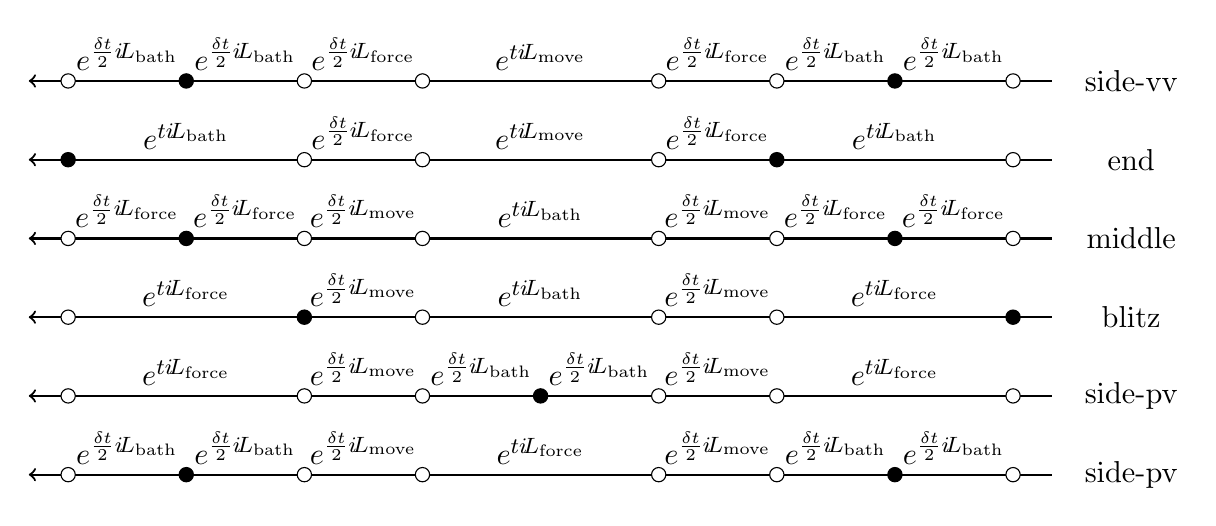
\begin{tikzpicture}
	% SIDE-VV:
	\draw[<-, thick] (0,5) -- (13,5);
%	\node() at (0,5)[left]{t};
	\node() at ( 0.5,5)[fill=white,shape=circle,draw,scale=0.5]{};
	\node() at ( 2.0,5)[fill=black,shape=circle,draw,scale=0.5]{};
	\node() at ( 3.5,5)[fill=white,shape=circle,draw,scale=0.5]{};
	\node() at ( 5.0,5)[fill=white,shape=circle,draw,scale=0.5]{};
	\node() at ( 8.0,5)[fill=white,shape=circle,draw,scale=0.5]{};
	\node() at ( 9.5,5)[fill=white,shape=circle,draw,scale=0.5]{};
	\node() at (11.0,5)[fill=black,shape=circle,draw,scale=0.5]{};
	\node() at (12.5,5)[fill=white,shape=circle,draw,scale=0.5]{};
	\node() at ( 1.25,5)[above] {$e^{\frac{\delta t}{2} \Liu_\mathrm{bath}}$};
	\node() at ( 2.75,5)[above] {$e^{\frac{\delta t}{2} \Liu_\mathrm{bath}}$};
	\node() at ( 4.25,5)[above] {$e^{\frac{\delta t}{2} \Liu_\mathrm{force}}$};
	\node() at ( 6.50,5)[above] {$e^{t \Liu_\mathrm{move}}$};
	\node() at ( 8.75,5)[above] {$e^{\frac{\delta t}{2} \Liu_\mathrm{force}}$};
	\node() at (10.25,5)[above] {$e^{\frac{\delta t}{2} \Liu_\mathrm{bath}}$};
	\node() at (11.75,5)[above] {$e^{\frac{\delta t}{2} \Liu_\mathrm{bath}}$};
	\node() at (14,5)[] {side-vv};

	% END
	\draw[<-, thick] (0,4) -- (13,4);
%	\node() at (0,4)[left]{t};
	\node() at ( 0.5,4)[fill=black,shape=circle,draw,scale=0.5]{};
	\node() at ( 3.5,4)[fill=white,shape=circle,draw,scale=0.5]{};
	\node() at ( 5.0,4)[fill=white,shape=circle,draw,scale=0.5]{};
	\node() at ( 8.0,4)[fill=white,shape=circle,draw,scale=0.5]{};
	\node() at ( 9.5,4)[fill=black,shape=circle,draw,scale=0.5]{};
	\node() at (12.5,4)[fill=white,shape=circle,draw,scale=0.5]{};
	\node() at ( 2.00,4)[above] {$e^{t \Liu_\mathrm{bath}}$};
	\node() at ( 4.25,4)[above] {$e^{\frac{\delta t}{2} \Liu_\mathrm{force}}$};
	\node() at ( 6.50,4)[above] {$e^{t \Liu_\mathrm{move}}$};
	\node() at ( 8.75,4)[above] {$e^{\frac{\delta t}{2} \Liu_\mathrm{force}}$};
	\node() at (11.00,4)[above] {$e^{t \Liu_\mathrm{bath}}$};
	\node() at (14,4)[] {end};

	% MIDLLE
	\draw[<-, thick] (0,3) -- (13,3);
%	\node() at (0,3)[left]{t};
	\node() at ( 0.5,3)[fill=white,shape=circle,draw,scale=0.5]{};
	\node() at ( 2.0,3)[fill=black,shape=circle,draw,scale=0.5]{};
	\node() at ( 3.5,3)[fill=white,shape=circle,draw,scale=0.5]{};
	\node() at ( 5.0,3)[fill=white,shape=circle,draw,scale=0.5]{};
	\node() at ( 8.0,3)[fill=white,shape=circle,draw,scale=0.5]{};
	\node() at ( 9.5,3)[fill=white,shape=circle,draw,scale=0.5]{};
	\node() at (11.0,3)[fill=black,shape=circle,draw,scale=0.5]{};
	\node() at (12.5,3)[fill=white,shape=circle,draw,scale=0.5]{};
	\node() at ( 1.25,3)[above] {$e^{\frac{\delta t}{2} \Liu_\mathrm{force}}$};
	\node() at ( 2.75,3)[above] {$e^{\frac{\delta t}{2} \Liu_\mathrm{force}}$};
	\node() at ( 4.25,3)[above] {$e^{\frac{\delta t}{2} \Liu_\mathrm{move}}$};
	\node() at ( 6.50,3)[above] {$e^{t \Liu_\mathrm{bath}}$};
	\node() at ( 8.75,3)[above] {$e^{\frac{\delta t}{2} \Liu_\mathrm{move}}$};
	\node() at (10.25,3)[above] {$e^{\frac{\delta t}{2} \Liu_\mathrm{force}}$};
	\node() at (11.75,3)[above] {$e^{\frac{\delta t}{2} \Liu_\mathrm{force}}$};
	\node() at (14,3)[] {middle};

	% BLITZ
	\draw[<-, thick] (0,2) -- (13,2);
%	\node() at (0,2)[left]{t};
	\node() at ( 0.5,2)[fill=white,shape=circle,draw,scale=0.5]{};
	\node() at ( 3.5,2)[fill=black,shape=circle,draw,scale=0.5]{};
	\node() at ( 5.0,2)[fill=white,shape=circle,draw,scale=0.5]{};
	\node() at ( 8.0,2)[fill=white,shape=circle,draw,scale=0.5]{};
	\node() at ( 9.5,2)[fill=white,shape=circle,draw,scale=0.5]{};
	\node() at (12.5,2)[fill=black,shape=circle,draw,scale=0.5]{};
	\node() at ( 2.00,2)[above] {$e^{t \Liu_\mathrm{force}}$};
	\node() at ( 4.25,2)[above] {$e^{\frac{\delta t}{2} \Liu_\mathrm{move}}$};
	\node() at ( 6.50,2)[above] {$e^{t \Liu_\mathrm{bath}}$};
	\node() at ( 8.75,2)[above] {$e^{\frac{\delta t}{2} \Liu_\mathrm{move}}$};
	\node() at (11.00,2)[above] {$e^{t \Liu_\mathrm{force}}$};
	\node() at (14,2)[] {blitz};

	% SIDE-PV 1
	\draw[<-, thick] (0,1) -- (13,1);
%	\node() at (0,1)[left]{t};
	\node() at ( 0.5,1)[fill=white,shape=circle,draw,scale=0.5]{};
	\node() at ( 3.5,1)[fill=white,shape=circle,draw,scale=0.5]{};
	\node() at ( 5.0,1)[fill=white,shape=circle,draw,scale=0.5]{};
	\node() at ( 6.5,1)[fill=black,shape=circle,draw,scale=0.5]{};
	\node() at ( 8.0,1)[fill=white,shape=circle,draw,scale=0.5]{};
	\node() at ( 9.5,1)[fill=white,shape=circle,draw,scale=0.5]{};
	\node() at (12.5,1)[fill=white,shape=circle,draw,scale=0.5]{};
	\node() at ( 2.00,1)[above] {$e^{t \Liu_\mathrm{force}}$};
	\node() at ( 4.25,1)[above] {$e^{\frac{\delta t}{2} \Liu_\mathrm{move}}$};
	\node() at ( 5.75,1)[above] {$e^{\frac{\delta t}{2} \Liu_\mathrm{bath}}$};
	\node() at ( 7.25,1)[above] {$e^{\frac{\delta t}{2} \Liu_\mathrm{bath}}$};
	\node() at ( 8.75,1)[above] {$e^{\frac{\delta t}{2} \Liu_\mathrm{move}}$};
	\node() at (11.00,1)[above] {$e^{t \Liu_\mathrm{force}}$};
	\node() at (14,1)[] {side-pv};

	% SIDE-PV 2
	\draw[<-, thick] (0,0) -- (13,0);
%	\node() at (0,0)[left]{t};
	\node() at ( 0.5,0)[fill=white,shape=circle,draw,scale=0.5]{};
	\node() at ( 2.0,0)[fill=black,shape=circle,draw,scale=0.5]{};
	\node() at ( 3.5,0)[fill=white,shape=circle,draw,scale=0.5]{};
	\node() at ( 5.0,0)[fill=white,shape=circle,draw,scale=0.5]{};
	\node() at ( 8.0,0)[fill=white,shape=circle,draw,scale=0.5]{};
	\node() at ( 9.5,0)[fill=white,shape=circle,draw,scale=0.5]{};
	\node() at (11.0,0)[fill=black,shape=circle,draw,scale=0.5]{};
	\node() at (12.5,0)[fill=white,shape=circle,draw,scale=0.5]{};
	\node() at ( 1.25,0)[above] {$e^{\frac{\delta t}{2} \Liu_\mathrm{bath}}$};
	\node() at ( 2.75,0)[above] {$e^{\frac{\delta t}{2} \Liu_\mathrm{bath}}$};
	\node() at ( 4.25,0)[above] {$e^{\frac{\delta t}{2} \Liu_\mathrm{move}}$};
	\node() at ( 6.50,0)[above] {$e^{t \Liu_\mathrm{force}}$};
	\node() at ( 8.75,0)[above] {$e^{\frac{\delta t}{2} \Liu_\mathrm{move}}$};
	\node() at (10.25,0)[above] {$e^{\frac{\delta t}{2} \Liu_\mathrm{bath}}$};
	\node() at (11.75,0)[above] {$e^{\frac{\delta t}{2} \Liu_\mathrm{bath}}$};
	\node() at (14,0)[] {side-pv};
\end{tikzpicture}

	\caption{Integration schemes.
	In all schemes, force computation is required once per time step.}
	\label{fig:STS integration schemes}
\end{figure*}

Fig.~\ref{fig:STS integration schemes} also shows that the time-reversible middle scheme is truly distinct from the previous ones.
If its difficulty to keep the canonical distribution of momenta is really due to the sampling's precedence by a force-induced transformation, then a simple shift of endpoints can possibly solve the problem.
Such shift is the one that results in
\begin{multline}
\label{eq:STS blitz scheme propagator}
e^{t \Liu_\mathrm{blitz}} = \Big[
e^{\frac{t}{2n} \Liu_\mathrm{move}}
e^{\frac{t}{n} \Liu_\mathrm{bath}}
e^{\frac{t}{2n} \Liu_\mathrm{move}}
e^{\frac{t}{n} \Liu_\mathrm{force}}
\Big]^{n},
\end{multline}
which is also represented in Fig.~\ref{fig:STS integration schemes}.
The name blitz is meant to remind that the forces are employed fully at the onset of every step.
As one can observe, this method can produce the same overall trajectory and the same coordinate samples as the middle scheme.
However, the momentum values resulting from the action of the thermostat will remain untouched until sampling.
Like the end scheme, the new method is not time-reversible, but the importance of such feature depends on the desired application.
For instance, it is very important for the design of a Hybrid Monte Carlo method, but it might be unnecessary for simple Molecular Dynamics sampling.

Finally, it is possible to devise another method with both time-reversal symmetry and overall-trajectory correspondence to the middle scheme.
This is done by moving the step endpoint to halfway into the thermostat integration.
In Fig.~\ref{fig:STS integration schemes}, this scheme is referred to as side-pv.
To explain why, we show a second representation of the same method, so as to facilitate a direct comparison with the side-vv scheme.
Note that side-pv could have derived from side-vv by replacing its Velocity-Verlet core by a Position-Verlet integrator \cite{Tuckerman_1992}.
Despite the overall-trajectory correspondence, the middle and side-pv schemes produce distinct samples in terms of both coordinates and momenta.
By applying the reasoning employed thus far to compare the three time-reversible schemes, side-pv is expected to yield better coordinates but worse momenta than side-vv, as well as better momenta but worse coordinates than the middle scheme.

\subsection{Multiple Time Scale Integration}

There are many possible ways of generalizing the methods discussed in the previous section and devising a multiple time-scale (MTS) integration procedure.
However, we adopt here some restraints to avoid excessive intricacy.
To come up with a MTS integration scheme using the reference system propagator algorithm (RESPA) \cite{Tuckerman_1992}, we split the force on each degree of freedom $\dof$ into a sum of $M$ terms, i.e. $F_\dof = \sum_{k=1}^M F_\dof^k$.
The characteristic time scale of each force component increases with index $k$, meaning that $F_\dof^1$ is the fastest component while $F_\dof^M$ is the slowest one.
In the basic RESPA recipe, integration at the largest time scale ($k=M$) is done by executing $n_M$ steps of size $\delta t_M = \Delta t$.
Internally, every step of size $\delta t_k$, taken at a time scale $k$, involves $n_{k-1}$ substeps of size $\delta t_k/n_{k-1}$ each.

In general, coordinate moves are performed at the same time scale of the fastest forces.
It is possible, though, to factorize them even further, especially if they are interwoven with the handling of extended space variables.
This is done, for instance, when the coordinate moves are required to follow a geodesic motion through a constrained manifold \cite{Leimkuhler_2016}.
For simplicity, however, we will not consider this possibility in our formulation.

This time, let us partition the extended phase-space Liouville operator in Eq.~\eqref{eq:general equation of motion} as
\begin{equation}
\label{eq:RESPA Liouville Partition}
\Liu = \Liu_\mathrm{move} + \sum_{k=1}^M \Liu_\mathrm{force}^k + \sum_{k=0}^M \Liu_\mathrm{bath}^k,
\end{equation}
where, like in Eq.~\eqref{eq:STS Liouville Partition}, a given component $\Liu_\mathrm{force}^k$ is the only one that depends on the forces labeled with superscript $k$, while operators $\{\Liu_\mathrm{bath}^k\}_{k=0}^M$ are reserved for transformations in particle momenta affected by extended phase-space variables exclusively.
The classical propagator representing a relatively general RESPA scheme can be written in a recursive manner as
\begin{equation}
\label{eq:RESPA outermost propagator}
e^{t \Liu} \approx \mathcal{G}_M(t),
\end{equation}
where $\mathcal{G}_M$ belongs to a family of operators whose each member $\mathcal{G}_k(\delta t)$ for $k \in [1, M]$ is
\begin{multline}
\label{eq:RESPA scheme 1}
\mathcal{G}_k(\delta t) = \Big[
e^{\frac{\delta t}{2 n_k} \Liu_\mathrm{bath}^k}
e^{\frac{\delta t}{2 n_k} \Liu_\mathrm{force}^k}
\mathcal{G}_{k-1}\left(\tfrac{\delta t}{n_k}\right)
\times \\ \times
e^{\frac{\delta t}{2 n_k} \Liu_\mathrm{force}^k}
e^{\frac{\delta t}{2 n_k} \Liu_\mathrm{bath}^k}
\Big]^{n_k}.
\end{multline}

Finally, the recursive process comes to an end once we make
\begin{equation}
\label{eq:RESPA innermost propagator}
\mathcal{G}_0(\delta t) = e^{\frac{\delta t}{2} \Liu_\mathrm{move}}
e^{\delta t \Liu_\mathrm{bath}^0}
e^{\frac{\delta t}{2} \Liu_\mathrm{move}}.
\end{equation}

In this general formulation, one is free to allocate the components of $\Liu_\mathrm{bath}$ throughout the several time scales, provided that $\sum_{k=0}^M \Liu_\mathrm{bath}^k = \Liu_\mathrm{bath}$.
For simplicity, however, we only consider cases in which the whole integration is done in a single time scale with selected index $k^\ast$, thus making $\Liu_\mathrm{bath}^k = 0$ for all $k \neq k^\ast$.
When $k^\ast \geq 1$, we can conveniently rewrite Eq.~\eqref{eq:RESPA innermost propagator} as $\mathcal{G}_0(\delta t) = e^{\delta t \Liu_\mathrm{move}}$.

Our formulation reproduces the XO-RESPA (extended system outside-RESPA) method introduced in Ref.~\citenum{Martyna_1996} if $k^\ast = M$.
Although the XI-RESPA (extended system inside-RESPA) scheme \cite{Martyna_1996} does not fit exactly into the present notation, a close variant XI\textsuperscript{*}-RESPA can be devised if we make $k^\ast = 1$.
Both XO-RESPA and XI-RESPA can be considered as MTS generalizations of the side-vv scheme of Fig.~\ref{fig:STS integration schemes}.

An important innovation, considering the findings of Zhang and coworkers \cite{Zhang_2017}, is that the proposed formulation becomes a MTS generalization of the middle scheme (Fig.~\ref{fig:STS integration schemes}) if we simply make $k^\ast = 0$.

Finally, in an attempt to generalize the blitz scheme, 

\begin{equation}
\label{eq:RESPA scheme 2}
\mathcal{G}_k(\delta t) = \Big[
\mathcal{G}_{k-1}\left(\tfrac{\delta t}{n_k}\right)
e^{\frac{\delta t}{n_k} \Liu_\mathrm{force}^k}
\Big]^{n_k}.
\end{equation}

\subsection{Massive Nos\'e-Hoover-Langevin Dynamics}

In order to compare the several splitting strategies, we employ a massive-thermostat variant of the Nos\'e-Hoover-Langevin method \cite{Samoletov_2007, Leimkuhler_2009}, referred to here as NHL(R).
As in Ref.~\citenum{Leimkuhler_2013}, the R stands for a possible RESPA-type integration.
The system motion is, in this case, described by the stochastic differential equation (SDE) system
\begin{subequations}
	\label{eq:NHL equations of motion}
	\begin{align}
	& dq_\dof = v_\dof dt, \label{eq:NHL q} \\
	& dv_\dof = \frac{F_\dof}{m_\dof} dt - v_{2,\dof} v_\dof dt, \quad \mathrm{and} \label{eq:NHL v}  \\
	& dv_{2,\dof} = \tfrac{m_\dof v_\dof^2 - kT}{Q_2}dt - \gamma v_{2,\dof} dt + \sqrt{\tfrac{2 \gamma kT}{Q_2}} dW_\dof, \label{eq:NHL v2}
	\end{align}
\end{subequations}
where $\gamma$ is a friction constant and $dW_\dof$ represents an infinitesimal increment of a stochastic Wiener process.
The inertial parameter $Q_2$ is the same for all degrees of freedom and, as usual, it is computed by $Q_2 = kT\tau^2$, where $\tau$ is a relevant time scale of the system dynamics.
We can formally express a solution of this system as $x(t) = e^{t \Liu_\mathrm{NHL(R)}} x_0$, where
\begin{multline}
\label{eq:NHL Liouville operator}
\Liu_\mathrm{NHL(R)} = \sum_\dof \bigg[ v_\dof \diff{q_\dof}{} + \\
+ \left(\frac{F_\dof}{m_\dof} - v_{2,\dof} v_\dof \right) \diff{v_\dof}{} \bigg] + \Liu_\mathrm{DOU}
\end{multline}
and $\Liu_\mathrm{DOU}$ is the operator which, alone, generates a drifted Ornstein-Uhlenbeck process whose motion is given, for every defree of freedom $\dof$, by $dq_\dof = 0$, $dv_\dof = 0$, and
\begin{equation}
\label{eq:DOU equation of motion}
dv_{2,\dof} = \gamma (\mu_\dof - v_{2,\dof}) dt + \sqrt{\tfrac{2 \gamma kT}{Q_2}} dW_\dof,
\end{equation}
where $\mu_\dof = \frac{m_\dof v_\dof^2 - kT}{\gamma Q_2}$ is a constant drift.
It is possible to solve the equation above by carrying out an It\={o} integration \cite{Leimkuhler_2015} after multiplying both sides by $e^{\gamma t}$, thus yielding
\begin{multline*}
v_{2,\dof}(\delta t) = v_{2,\dof}^0 e^{-\gamma \delta t} +
\mu_\dof (1 - e^{-\gamma \delta t}) + \\
+ \sqrt{\tfrac{kT}{Q_2}(1 - e^{-2\gamma \delta t})} R_n(\delta t),
\end{multline*}
where $R_n(t)$ evaluates to a standard normal random deviate at any time $t$.

In our strategy for numerically evaluating propagator $e^{t \Liu_\mathrm{NHL(R)}}$, we employ Eq.~\eqref{eq:RESPA Liouville Partition} with
\begin{equation}
\Liu_\mathrm{move} = \sum_\dof v_\dof \diff{q_\dof}{},
\end{equation}
meaning that the effect of propagator $e^{\delta t \Liu_\mathrm{move}}$ is a simple translation $q_\dof \leftarrow q_\dof + v_\dof \delta t$ for all $\dof$, and
\begin{equation}
\Liu_\mathrm{force}^k = \sum_\dof \frac{F_\dof^k}{m_\dof} \diff{v_\dof}{},
\end{equation}
which yields a simple boost $v_\dof \leftarrow v_\dof + \frac{F_\dof^k}{m_\dof} \delta t$ for all $\dof$ as the action of propagator $e^{\delta t \Liu_\mathrm{force}^k}$.
Therefore, $\Liu_\mathrm{bath}$ contains the remaining components of the overall Liouville operator.
We express it as $\Liu_\mathrm{bath} = \Liu_\mathrm{scaling} + \Liu_\mathrm{DOU}$, where
\begin{equation}
\Liu_\mathrm{scaling} = -\sum_\dof v_{2,\dof} v_\dof \diff{v_\dof}{},
\end{equation}
so that the solution of $e^{\delta t \Liu_\mathrm{scaling}}$ alone is a scaling of velocities given by $v_\dof(t) = v_\dof^0 e^{-v_{2,\dof} \delta t}$ for all $\dof$.
Since the full propagator $e^{\delta t \Liu_\mathrm{bath}}$ does not allow a simple analytical solution, we employ a Trotter-Suzuki splitting in the form
\begin{equation*}
e^{\delta t \Liu_\mathrm{bath}} \approx
e^{\frac{\delta t}{2} \Liu_\mathrm{scaling}}
e^{\delta t \Liu_\mathrm{DOU}}
e^{\frac{\delta t}{2} \Liu_\mathrm{scaling}}.
\end{equation*}

\subsection{Stochastic Isokinetic Nos\'e-Hoover Method}

In the SIN(R) method, we define a pair of extended-system variables $v_{1,\dof}$ and $v_{2,\dof}$ for every dof $\dof$, with associated inertial parameters $Q_1$ and $Q_2$, respectively.
In practice, a single and common value $Q_1 = Q_2 = kT\tau^2$ is employed.
The SDE system which prescribes the dynamics of the SIN(R) method is
\begin{subequations}
	\label{eq:SINR equations of motion}
	\begin{align}
	& dq_\dof = v_\dof dt, \label{eq:SINR q} \\
	& dv_\dof = \frac{F_\dof}{m_\dof} dt - \lambda_\dof v_\dof dt, \quad \mathrm{and} \label{eq:SINR v}  \\
	& dv_{1,\dof} = -\lambda_\dof v_{1,\dof} dt - v_{2,\dof} v_{1,\dof} dt, \quad \mathrm{and} \label{eq:SINR v1}  \\
	& dv_{2,\dof} = \tfrac{Q_1 v_{1,\dof}^2 - kT}{Q_2}dt - \gamma v_{2,\dof} dt + \sqrt{\tfrac{2 \gamma kT}{Q_2}} dW_\dof, \label{eq:SINR v2}
	\end{align}
\end{subequations}
where $\lambda_\dof$ is a Lagrange multiplier introduced with the aim of imposing an isokinetic constraint to each degree of freedom, which is \cite{Leimkuhler_2013, Margul_2016}
\begin{subequations}
\label{eq:isokinetic constraint}
\begin{equation}
m v_\dof^2 + \frac{1}{2} Q_1 v_{1,\dof}^2 = kT.
\end{equation}

As this constraint implies that
\begin{equation}
\label{eq:isokinetic constraint derivative}
m v_\dof dv_\dof + \frac{1}{2} Q_1 v_{1,\dof}dv_{1,\dof} = 0,
\end{equation}
\end{subequations}
substitution of $dv_\dof$ and $dv_{1,\dof}$ from Eqs.~\eqref{eq:SINR v} and \eqref{eq:SINR v1} leads to
\begin{equation}
\lambda_\dof = \frac{F_\dof v_\dof - \frac{1}{2} Q_1 v_{2,\dof} v_{1,\dof}^2}{m_\dof v_\dof^2 + \frac{1}{2} Q_1 v_{1,\dof}^2}.
\end{equation}

Expressing a formal solution for this system as $x(t) = e^{t \Liu_\mathrm{SIN(R)}} x_0$ implies that
\begin{multline}
\label{eq:SINR Liouville operator}
\Liu_\mathrm{SIN(R)} = \sum_\dof \bigg[ v_\dof\diff{q_\dof}{} + \left(\frac{F_\dof}{m_\dof} - \lambda_\dof v_\dof\right)\diff{v_\dof}{} \\
- \left( \lambda_\dof v_{1,\dof} + v_{2,\dof} v_{1,\dof} \right) \diff{v_{1,\dof}}{} \bigg] + \Liu_\mathrm{DOU,1},
\end{multline}
where $\Liu_{DOU,1}$ generates a constant-drift Ornstein-Uhlenbeck process very similar to the one governed by Eq.~\eqref{eq:DOU equation of motion}, except that the drift is given by $\mu_{1,\dof} = \frac{Q_1 v_{1,\dof}^2 - kT}{\gamma Q_2}$.

As demonstrated in Ref.~\citenum{Leimkuhler_2013}, the SIN(R) dynamics is ergodic and preserves the isokinetic distribution.
The equations resemble a Nos\'{e}-Hoover-Langevin thermostat \cite{Samoletov_2007, Leimkuhler_2009}, with $v_{1,\dof}$ acting as intermediary between the system dof $\dof$ and a Langevin-type thermostat.
It is also possible to consider the simultaneous action of a set of $2L$ thermostat variables per dof \cite{Minary_2003, Minary_2003_2}.
Throughout this document, however, we only adopt the simplest case ($L=1$) because the method's efficacy has been verified to depend little on the choice of $L$ \cite{Leimkuhler_2013, Margul_2016}.

\paragraph{Force-Dependent Isokinetic Propagator}

The equations of motion that stem from the Liouville operator in Eq.~\eqref{eq:force-dependent Liouville operator} are
\begin{subequations}
\label{eq:force-dependent isokinetic equations}
\begin{align}
& \dot{v}_\dof = \frac{F^k_\dof}{m_\dof} - \lambda^k_\dof v_\dof \quad \mathrm{and} \\
& \dot{v}_{1,\dof} = - \lambda^k_\dof v_{1,\dof}.
\end{align}
	
In this case, for Eq.~\eqref{eq:isokinetic constraint derivative} to be satisfied, it is required that
\begin{equation}
\lambda^k_\dof = \frac{F^k_\dof v_\dof}{m_\dof v_\dof^2 + \frac{1}{2} Q_1 v_{1,\dof}^2}.
\end{equation}
\end{subequations}

\paragraph{Force-Independent Isokinetic Propagator}

\begin{equation}
\lambda^\ast_\dof = \frac{- \frac{1}{2} Q_1 v_{2,\dof} v_{1,\dof}^2}{m_\dof v_\dof^2 + \frac{1}{2} Q_1 v_{1,\dof}^2}.
\end{equation}

\paragraph{Differences from Leimkuhler \textit{et al}. (2013) \cite{Leimkuhler_2013}}

Highlight the differences between the present SIN(R) implementation and the original one.

\section{Results}


\begin{figure}
\includegraphics{single_time_scale_coordinates}
\caption{Single time scale methods.
	(a) Potential energy per molecule.
	(b) Atomic pressure.
	(c) Molecular pressure.}
\label{fig:STS coordinate properties}
\end{figure}

\begin{figure}
	\includegraphics{single_time_scale_momenta}
	\caption{Single time scale integration.
		Kinetic Temperature.}
	\label{fig:STS momentum properties}
\end{figure}

\section{Conclusion}


\begin{acknowledgement}

C.R.A.A. acknowledges the financial support of Petrobras (project code CENPES 16113).

\end{acknowledgement}

\bibliography{RESPA}

\end{document}